\documentclass{beamer}
\usetheme[numbering=fullbar]{focus}
\setbeamertemplate{mini frames}{}
\usepackage[labelformat=simple]{subfig}
\usepackage{graphicx}
\usepackage[export]{adjustbox}
\usepackage[version=4]{mhchem}
\usepackage{fix-cm}
\usepackage{multicol}
\usepackage{mathtools}
\renewcommand{\thesubfigure}{\relax}

\title{Analysis Tools for the \\Finite Element Method}
\subtitle{Math 693B: Advanced Computational PDE}
\author{Geneva Porter}
\titlegraphic{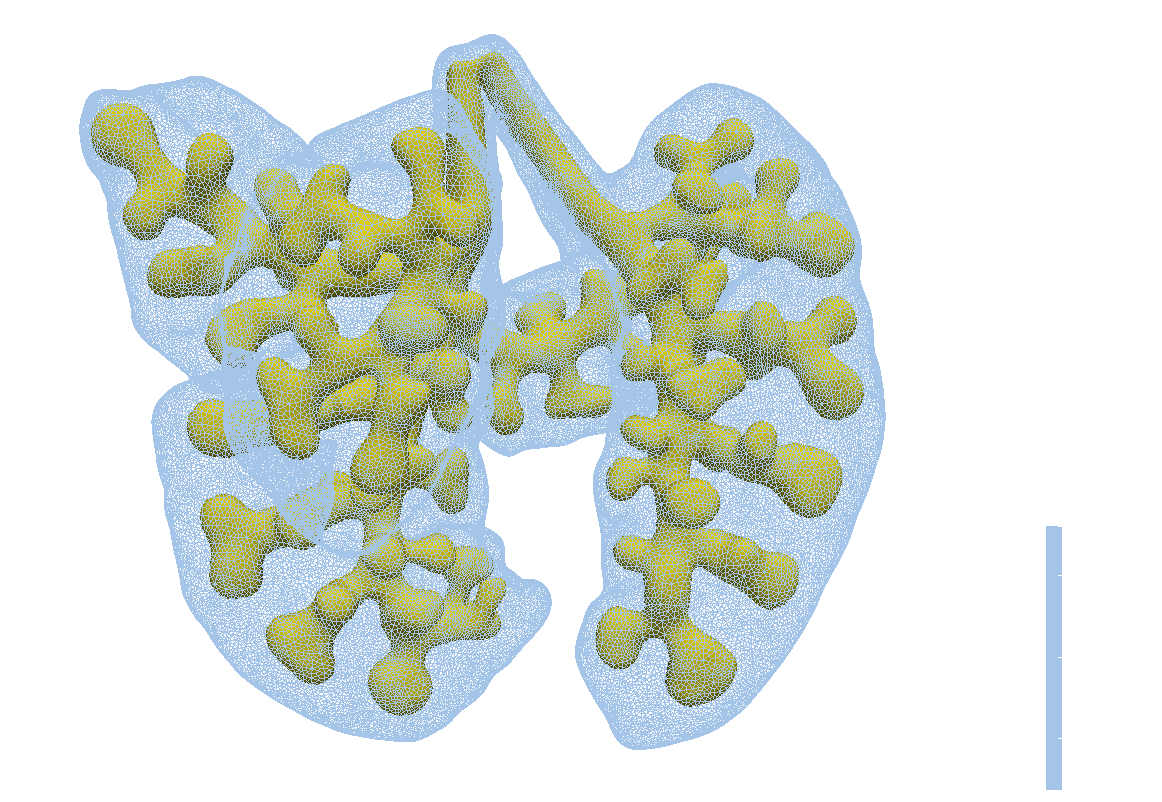
\includegraphics[height=4.7cm, trim=2cm 1cm 6cm 1cm , clip]{images/mesh_pretty.png}}
\institute{San Diego State University\\ Applied Mathematics}
\date{7 May 2020}

\begin{document}
\AtBeginSection{}

    \begin{frame}
        \maketitle
    \end{frame}

    
    \section[Introduction]{Introduction, Background, and Research Motivation}
    
        \begin{frame}{Reaction-Diffusion Models}    
            
			\begin{center}
				{\large Auto-catalytic Reaction Model}\\
				\vspace{-5mm}
				
				\begin{large}
					$$ \ce{X <=>[k_1][k_2] F} ~~~~~~~~~~ \ce{2F + S ->[k_3] 3F} ~~~~~~~~~~ \ce{Y ->[k_4] S} $$
				\end{large}
				
				
				\vspace{-5mm}
				
				{\Huge \textbf{+}} \\
				
				
				{\large Laplace-Beltrami Operator}\\
				\vspace{-5mm}
				
				\begin{equation*}
				\label{Laplace-Beltrami}
				\Delta_\Gamma u = \nabla_\Gamma\cdot\nabla_\Gamma u ~~~~~ \text{with} ~~~~~ \nabla_\Gamma u = \nabla u-(\nabla u\cdot\vec{n})\vec{n}
				\end{equation*}
				\vspace{-5mm}
				
				
				
				{\Huge \textbf{=}} \\
				
				
				{\large Schnakenberg Equations on Surface}\\
				\vspace{-5mm}
				
				\begin{equation*}
				\begin{aligned}
				& \dot{F} = \Delta_\Gamma F + 
				\gamma\left(\alpha - F + F^2S\right)\\
				& \dot{S} = \delta\Delta_\Gamma S + 
				\gamma\left(\beta - F^2S\right)\\
				\end{aligned}
				\end{equation*}
				
			\end{center}
		\end{frame}
	
		\begin{frame}{Lung Development}
		
		                \begin{figure}
			\centering
			
			\subfloat[Branching at the pseudoglandular stage]{\reflectbox{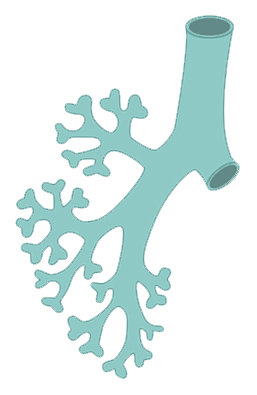
\includegraphics[width=3cm, height=4cm,frame]{images/lungs2.png}}}\qquad 
			\subfloat[Gene proteins diffuse from lung surface]{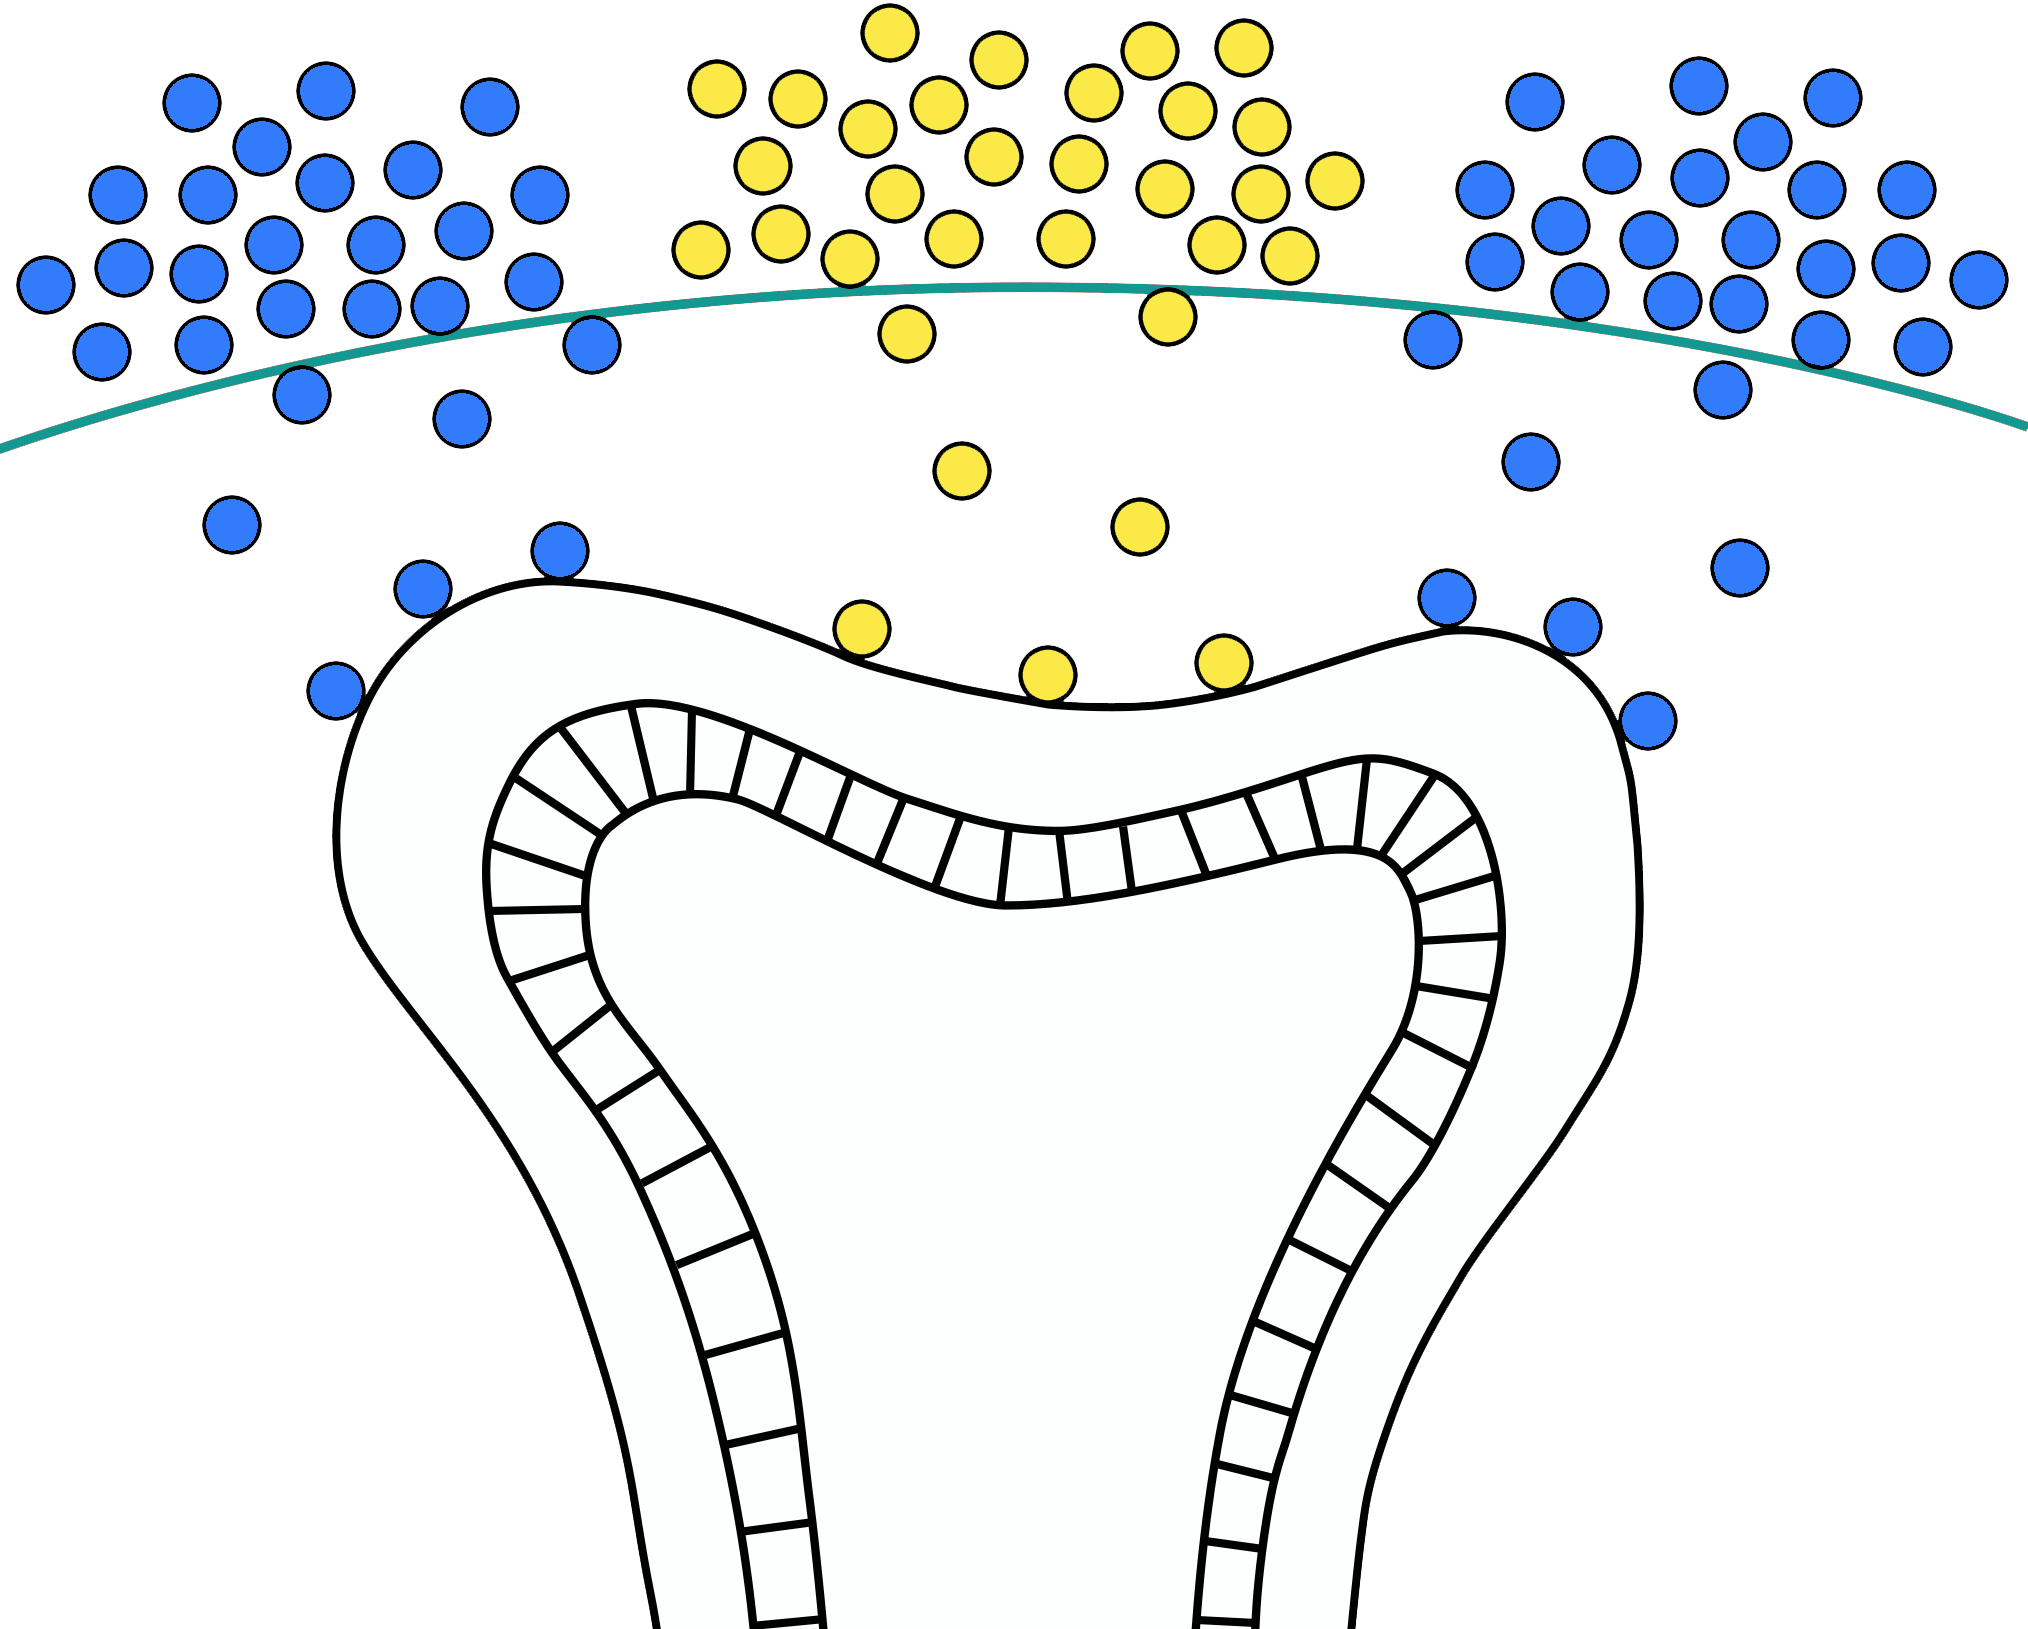
\includegraphics[width=3cm, height=4cm,frame]{images/lungs_diffusion2.png}}\qquad  \subfloat[Feedback loop between FGF10 and SHH genes]{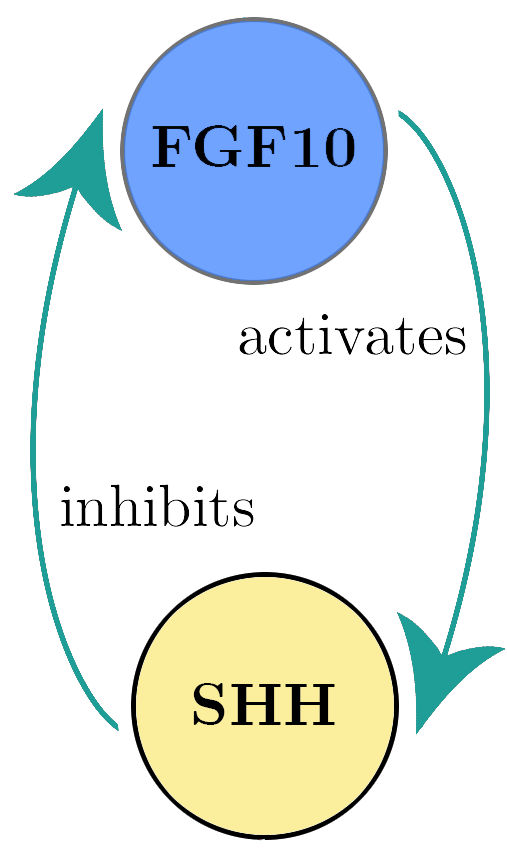
\includegraphics[width=3cm, height=4cm,frame]{images/feedback_loop2.png}}
			
		\end{figure}
			
		\end{frame}
	
		\begin{frame}{Sphere Study Validation}
		
		The problem is considered \textit{well posed}: existence, uniqueness, and continuity in initial data effects. The system is guaranteed to be well posed, since it is parabolic, has at least 2 boundary conditions and the spatial derivative is of the second degree \cite{Arnold2015}.
		
		\begin{figure}[H]\label{fig:mesh density}
			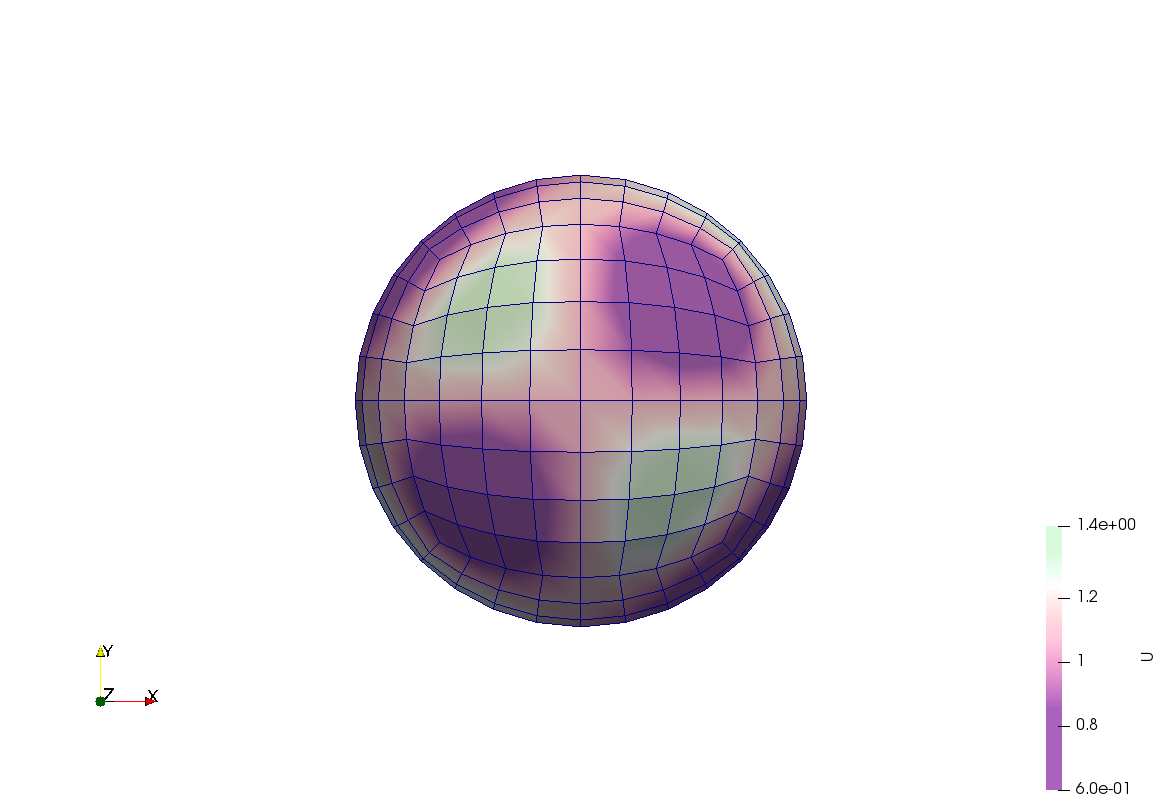
\includegraphics[width=.325\linewidth, trim= 10cm 5cm 10cm 5cm, clip]{images/ref2.png}
			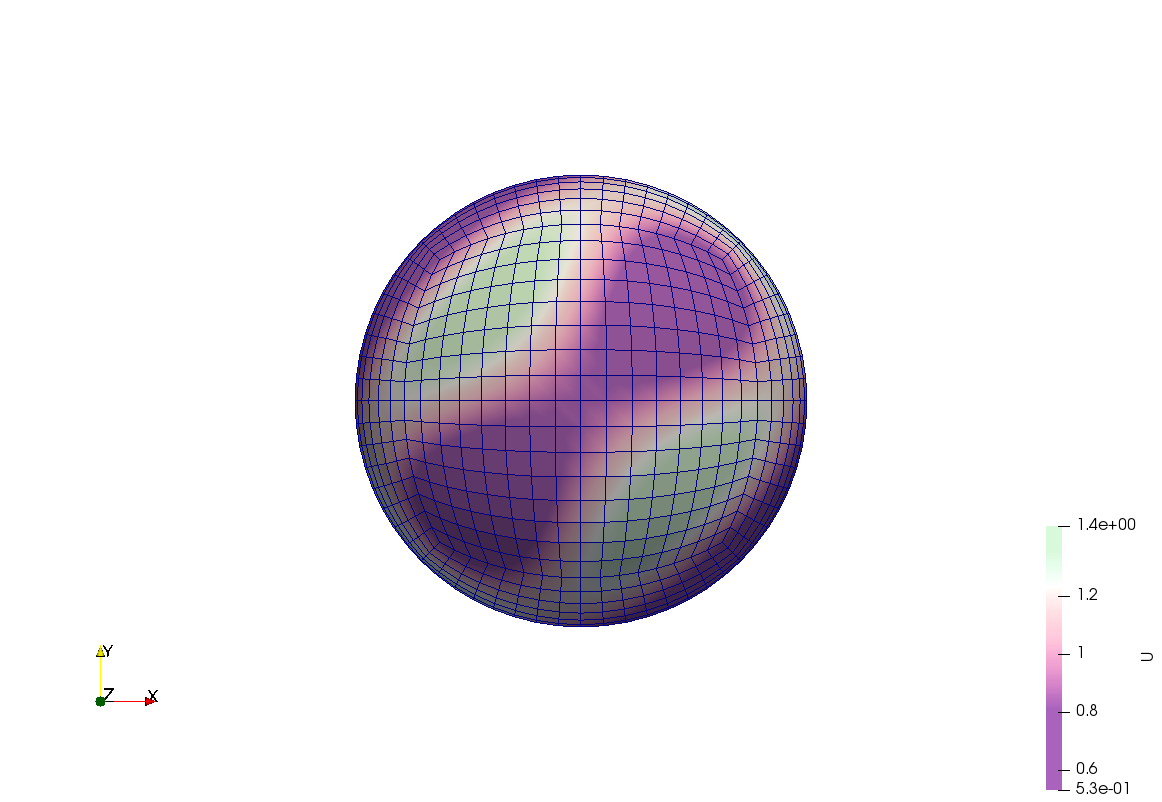
\includegraphics[width=.325\linewidth, trim= 10cm 5cm 10cm 5cm, clip]{images/ref3.png}
			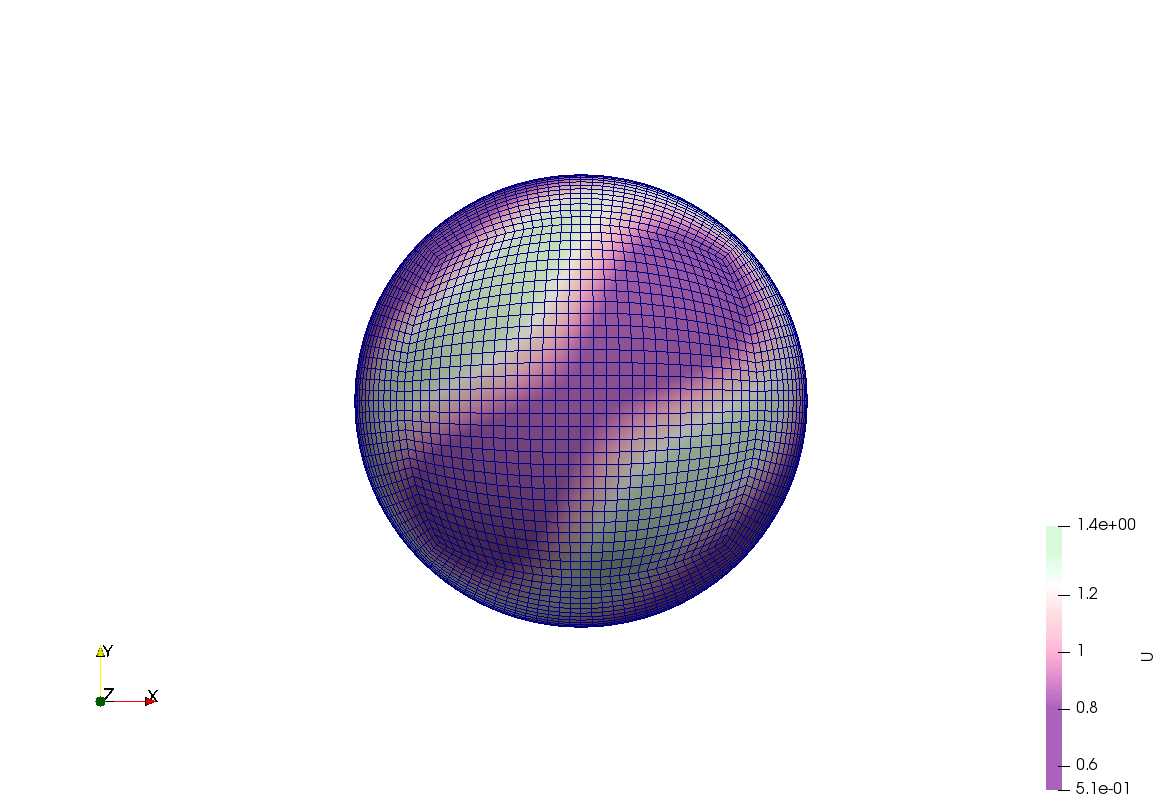
\includegraphics[width=.325\linewidth, trim= 10cm 5cm 10cm 5cm, clip]{images/ref4.png}
			\caption{Sphere meshes with density refinements $h_2$, $h_3$, and $h_4$}\label{fig:mesh_density}
		\end{figure}
		
		\end{frame}
    
    \section[FEM-IMEX]{Time and Space Discretization Schemes}
            
        \begin{frame}{The Finite Element Method}  
        
        Multiply by test function $\varphi$, integrate, and apply Green's Theorem:   
        
        \begin{equation*}\label{eq:weak2}
        \int_\Gamma \varphi\frac{\partial u}{\partial t} + \int_\Gamma \nabla_\Gamma\varphi\cdot\nabla_\Gamma u = \gamma\int_\Gamma \varphi f(u,v)
        \end{equation*} 
        
        Discretize the domain and the solution:        
        \begin{equation*}
        \begin{aligned}
        &\sum_j 
        \int_K \varphi_i\cdot\vartheta_j\left[\frac{\partial U_j}{\partial t}\right] + 
        \sum_j
        \int_K \nabla_K\varphi_i\cdot\nabla_K \vartheta_j \left[U_j\right]  &= 
        \gamma\sum_j
        \int_K \varphi_i f_K(U_j,V_j) 
        \end{aligned}
        \end{equation*}
        
        Simplify and substitute:        
        \begin{equation*}
        \begin{aligned}
        \textbf{M} = (\varphi_i,\varphi_j) ~~~~~~~~~~ \textbf{L} = (\nabla\varphi_i, \nabla\varphi_j) ~~~~~~~~~~ \textbf{A} = (\varphi_i,\textbf{a}) ~~~~~~~~~~ \textbf{B} = (\varphi_i,\textbf{b})
        \end{aligned}
        \end{equation*}        
        \begin{equation*}
        \begin{aligned}
        &\textbf{M}\cdot\frac{d}{dt}[U_j] + \textbf{L}\cdot U_j = \gamma (\textbf{A} - \textbf{M}\cdot U_j + \textbf{M}\cdot U_j^2V_j) 
        \end{aligned}
        \end{equation*}
                     
        \end{frame}
    
    	\begin{frame}{Implicit-Explicit Time Discretization}
    	
    	\vspace{-1cm}
    	
    	{\Large $$\textbf{M}\dot{U} + \textbf{L}U = \gamma\left[\textbf{A} - \textbf{M}U + \textbf{M}U^2V\right]$$}

    	\vspace{0mm}
    	
    	\begin{columns}
    		
    		\column{0.25\textwidth}    		
    		IMEX scheme, first order backward Euler:
    		
    		\column{0.75\textwidth}    		
    		$$ \frac{\textbf{M}(U_{n+1} - U_{n})}{k} + \textbf{L}U_{n+1} = \gamma\left(\textbf{A} - \textbf{M}U_{n+1} + \textbf{M}U_{n}^2V_{n}\right) $$
    		
    	\end{columns}
    \vfill
    	\begin{columns}    		
    		\column{0.25\textwidth}    		
    		Solve the linear system Ax=b:  
    		  		
    		\column{0.75\textwidth}    		
    		$$ \left[\frac{}{}(1+\gamma k)\textbf{M} + k \textbf{L}~\right]U_{n+1} = \gamma k\left(\frac{}{}\textbf{A} + \textbf{M}U_{n}^2V_{n}\right) $$
    		
    	\end{columns}
    \vfill
        	\begin{columns}    		
    	\column{0.25\textwidth}    		
    	Use the updated $u$ to solve $v$: 
    	
    	\column{0.75\textwidth}    		
    	$$ \left[\frac{}{}\textbf{M} + k\delta \textbf{A}~\right]V_{n+1} = \gamma k\left(\frac{}{}\textbf{B} - \textbf{M}U_{n+1}^2V_{n}\right) $$
    	
    	\end{columns}
    	
    \end{frame}
    
    \section[Error Analysis]{Consistency, Convergence, and Stability}
    
       \begin{frame}{Consistency}    
       
       The FDM normally shows consistency by solving:
       
       \begin{equation*}
       P\phi - P_{k,h}\phi \rightarrow 0 ~~~\text{as} ~~~ k,~h \rightarrow 0
       \end{equation*}   
       
       For the linearized system used in the FEM, we show consistency using the truncation error:
       
       \begin{equation*}\label{norm}
       \left|\left|\frac{}{} \gamma k\left(\frac{}{}\textbf{A} + \textbf{M}U_{n}^2V_{n}\right) - \left[\frac{}{}(1+\gamma k)\textbf{M} + k \textbf{L}~\right]U_{n+1}~ \right|\right| \lessapprox h^{p_1}+k^{p_2}
       \end{equation*} 
       
       Which gives an order of accuracy $(p_1, q_1)$. Because we use the \textbf{Conjugate Gradient Method}, we can constrain the truncation error to an arbitrary amount. For this model, we used $10^{-20}$.
           
       \end{frame}
   
	   \begin{frame}{Convergence}    
	   
	   Because of computing limitations, we use the criteria:
	      $$\left|\frac{}{} ||U_h|| - ||U_E|| ~\right| \leq \left|\frac{}{} || U_h - U_E|| ~ \right|  \lessapprox \left|h^{q_1} + k^{q_2}\right| = h^{q_1} + k^{q_2}$$
	      
	      with convergence rate $(q_1, q_2)$. Errors were compared with a domain of the same density but with $k=10^{-6}$.
	      \begin{figure}[H]
	      	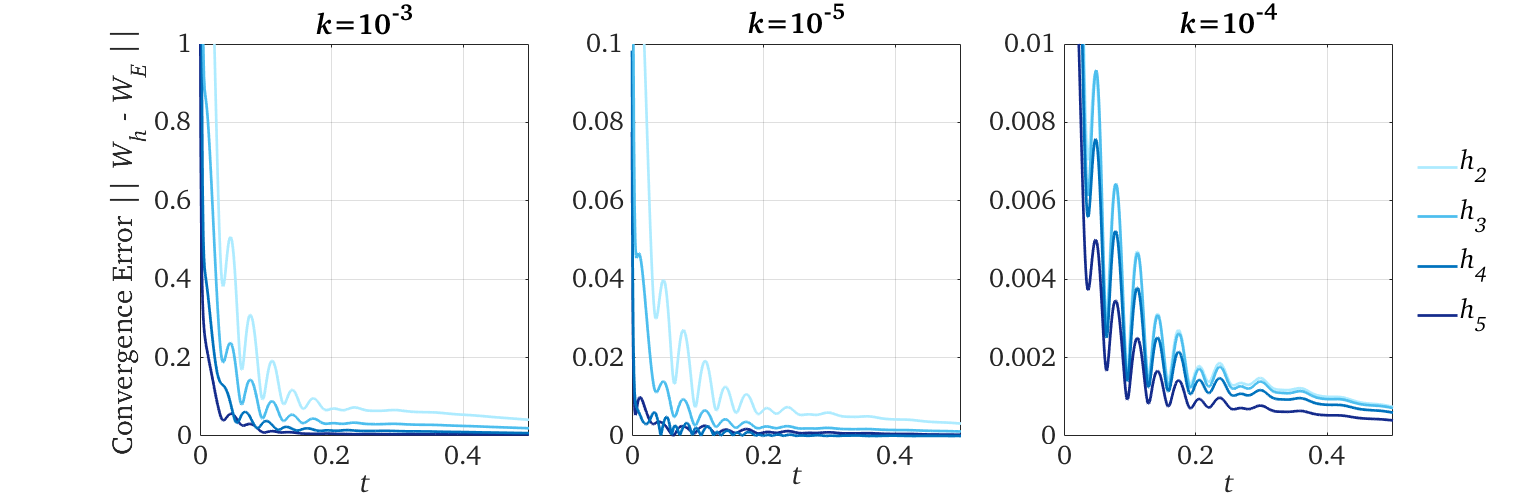
\includegraphics[width=.8\linewidth, trim=2.5cm 0 .5cm 0,clip]{images/norms_1.png}
	      	%\caption{Convergence norms for varying $h$ and $k$}\label{fig:convergence}
	      \end{figure}
      \centering All permutations converge, with the highest rate at (5, 5).
	   
		\end{frame}
		
		\begin{frame}{Stability}   
		
		\begin{theorem}[Lax-Richtmyer \cite{Dziuk2013}]
			Let $U_h$ be the solution of a numerical method consistent with a well-posed time-dependent problem; in particular, assume that it is accurate of order $p>0$. Then, if and only if the numerical method is stable, its solution converges with $p$th-order convergence rate,
			$$\left|\left|\frac{}{} U_h - U_E~\right|\right| \lessapprox \sum_{m=0}^n k\cdot ||\{\text{truncation error}\}|| \lessapprox h^{p_1} + k^{p_2}, ~~~t^n\in[0,T].$$
		\end{theorem}     
		
		\end{frame}
   
   \section[Discussion]{Results and Discussion}
   
   		\begin{frame}{Patterns on a Sphere}
   		
   		This analysis continues with studying how changing the parameters $\alpha,~ \beta, ~\delta, ~\text{and } \gamma$ influence the surface patterns.
   		
   		\vfill
   		
   			\begin{figure}[H]
   			\centering
   				\hspace*{\fill}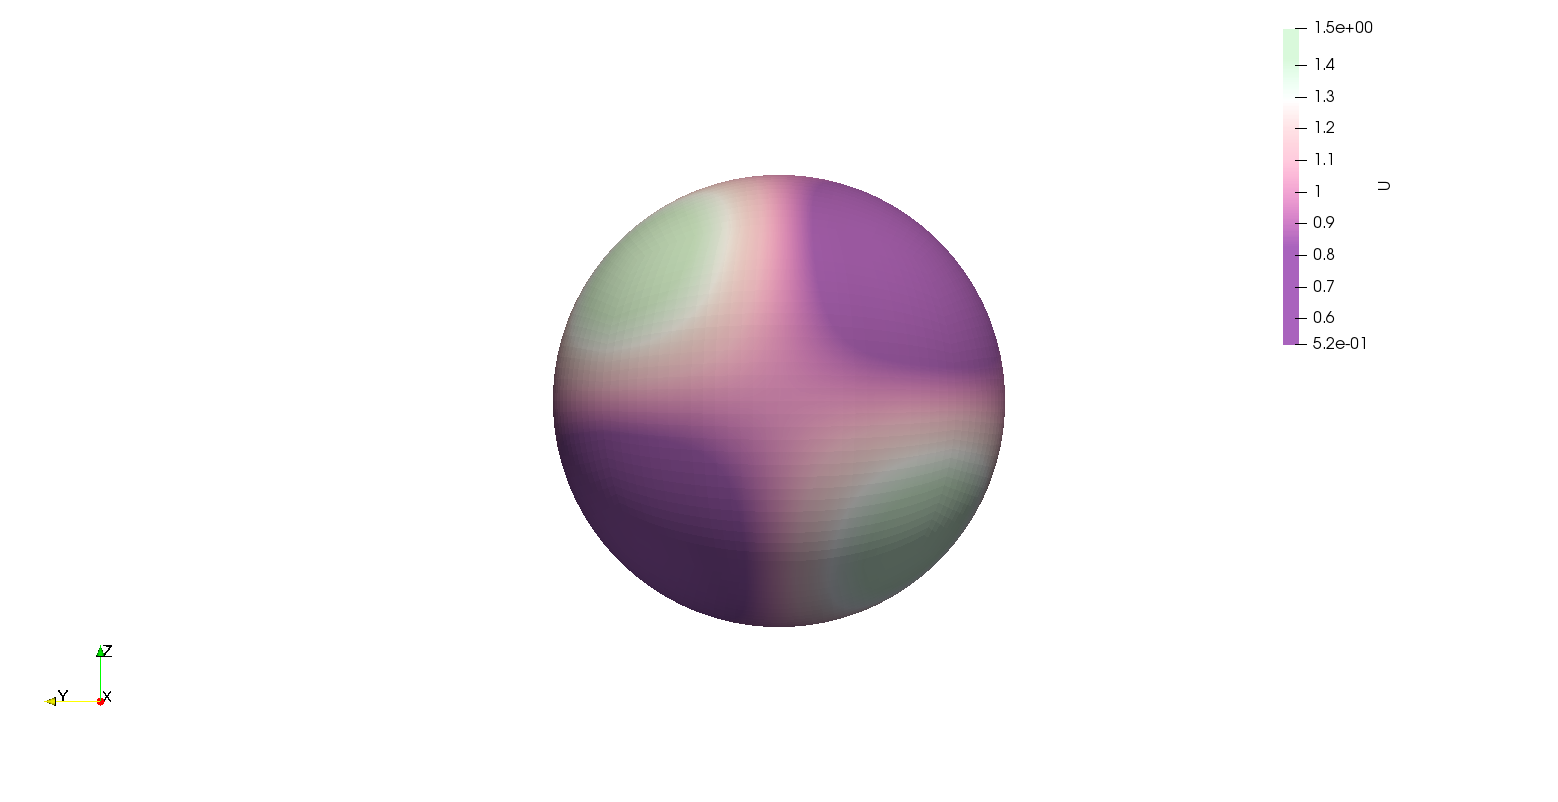
\includegraphics[width=.32\linewidth, trim = 18cm 6cm 18cm 6cm, clip]{images/compare-g-40-r-10.png}
   				\hspace*{\fill}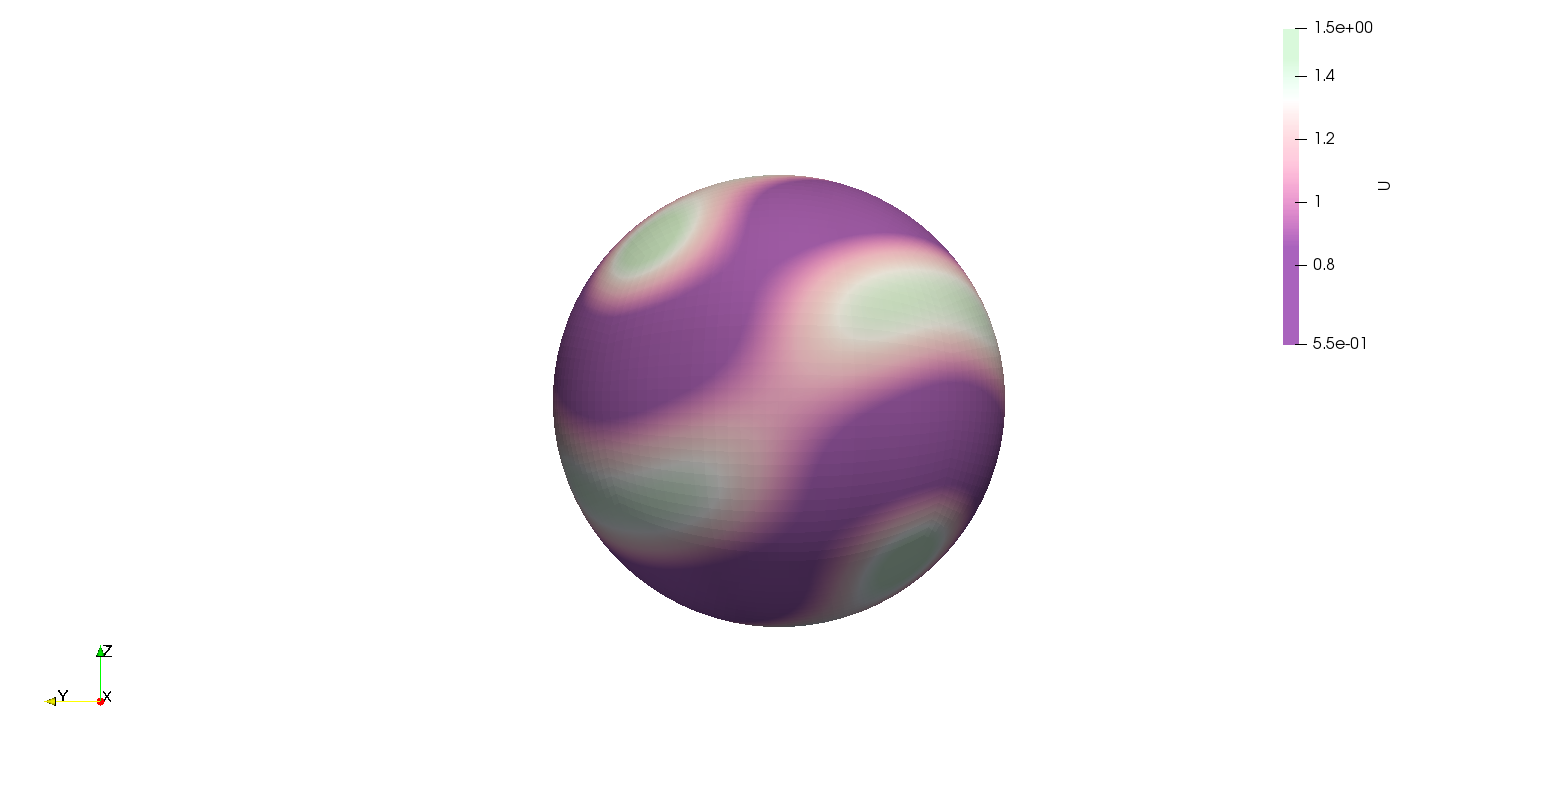
\includegraphics[width=.32\textwidth, trim = 18cm 6cm 18cm 6cm, clip]{images/compare-g-40-r-16.png}
   				\hspace*{\fill}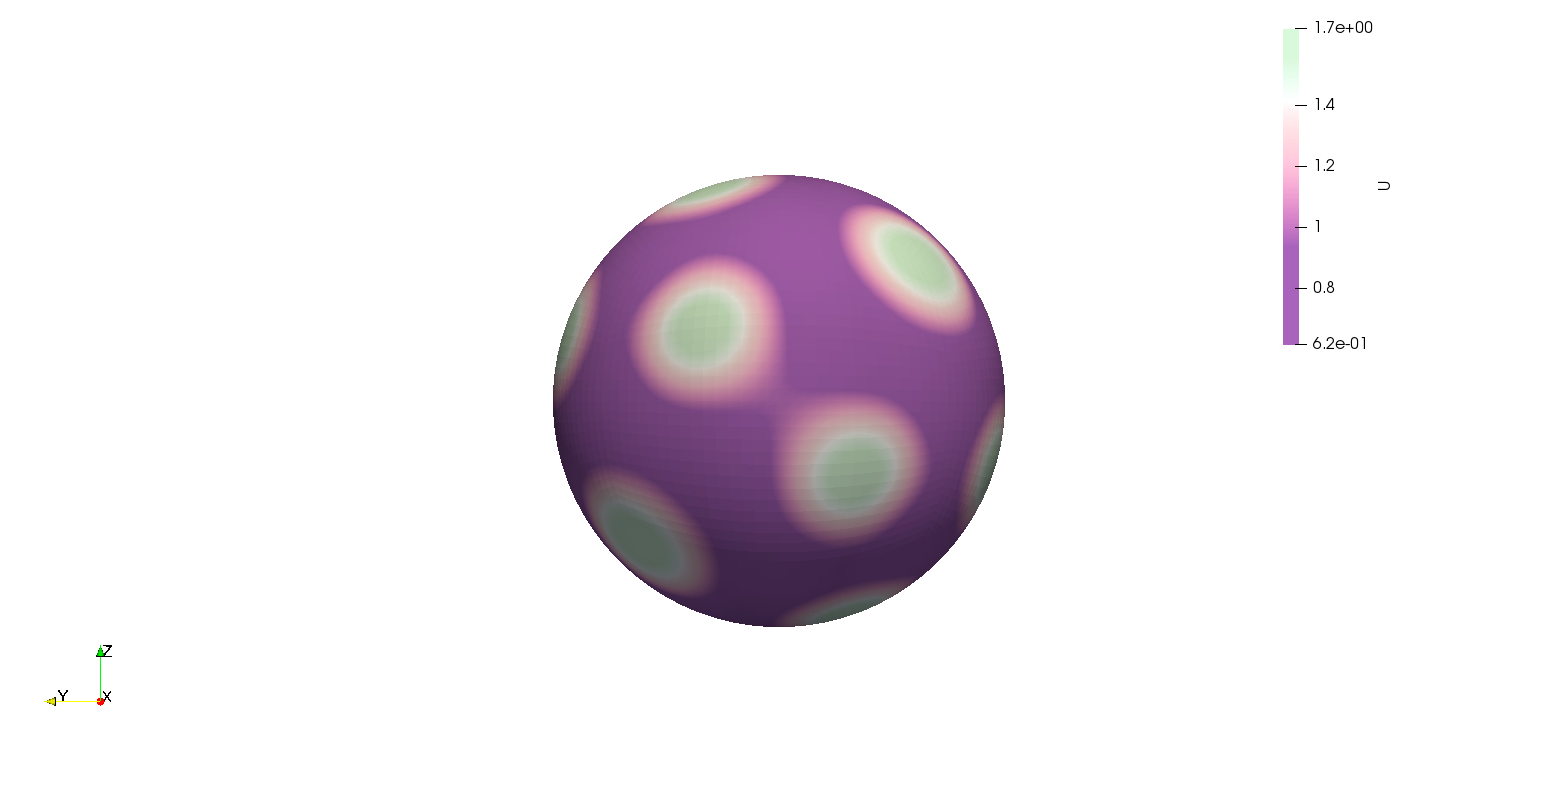
\includegraphics[width=.32\textwidth, trim = 18cm 6cm 18cm 6cm, clip]{images/compare-g-40-r-20.png}
   				\caption{Some examples of modeling various parameters}
   		\end{figure}
   		\end{frame}
   	
   		\begin{frame}{FGF-10 Distribution on the Lung}
   		
   		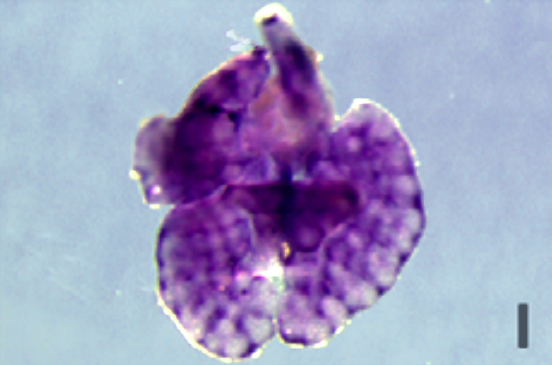
\includegraphics[width=.45\linewidth,trim=4cm 0 4cm 0, clip, frame]{images/mouse-lung-E13.5}\cite{Volckaert2013} \hfill
   		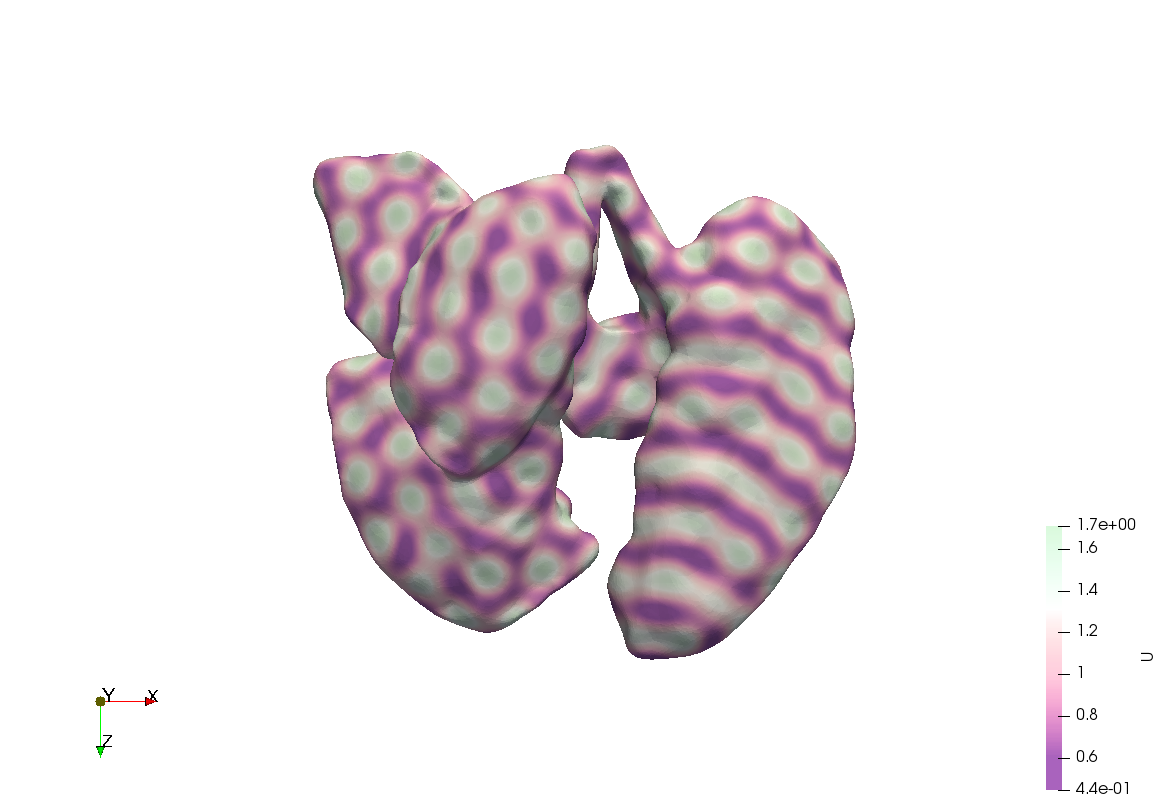
\includegraphics[width=.5\linewidth, trim=10cm 5cm 10cm 5cm, clip]{images/lung_example2.png}
   		
   		\end{frame}
            
            
            \appendix
            
            \begin{frame}{Further Reading}
                \nocite{*}
                \bibliography{short_bib}
                \bibliographystyle{ieeetr}
            \end{frame}
    
            \begin{frame}[focus]
                \huge Thank You!
            \end{frame}

    

\end{document}
